\section{Blind optimization: speedup without revelation}
\label{sec:blind-optimization}

We finally separate the two benefits that were bundled together in the
common-upper model.  Raw execution still takes the known time $u$, and one
unit of optimization still reduces the processing time to $p_i\in[0,u]$.
The difference is that optimization does not reveal $p_i$.  An optimized job
must be started blindly and its duration becomes known only when it finishes.
We call this the \emph{blind-optimization} model $\mathsf{BO}(u)$.

This small change removes the threshold decision entirely.  It also shows
that the bounded randomized ratio in the revealing model is genuinely an
information effect.

The goal of this section is to prove two closely related statements.  The
first, \cref{thm:bo-instance}, is the rigorous version of the informal
instance-optimality theorem \cref{thm:intro-bo-instance}.  The second,
\cref{thm:bo-curve}, is the rigorous version of
\cref{thm:intro-bo-curve} and maximizes that instance-specific value relative
to the clairvoyant optimum.  Keeping them together avoids repeating the same
two-block reduction.

For a multiset $M$ let
\[
 \mu_M=\frac1n\sum_{i=1}^n p_i
\]
and define
\begin{equation}
 \Phi_{\rm bo}(M)=\frac12\min\{u,1+\mu_M\}.
 \label{eq:bo-phi}
\end{equation}
The two terms have an immediate meaning.  Running every job raw uses $u$
units per completion.  Optimizing and then blindly processing every job uses
$1+\mu_M$ units per completion on average.

\begin{theorem}[Blind-optimization instance optimality]
\label{thm:bo-instance}
For every fixed $u<\infty$ there exist a randomized nonanticipating policy
$\mathcal A^{\rm bo}$, depending only on $n,u$, and a sequence
$\eps_u(n)\to0$ such that every size-$n$ multiset $M\subseteq[0,u]$ and every
fixed labeling $\sigma$ satisfy
\begin{equation}
 \EE C_{\mathcal A^{\rm bo}}(\sigma(M))
 \le n^2\Phi_{\rm bo}(M)+\eps_u(n)n^2.
 \label{eq:bo-instance-upper}
\end{equation}
Conversely, for every randomized nonanticipating policy $\mathcal A$, even
one told $M$, some fixed oblivious labeling $\sigma$ satisfies
\begin{equation}
 \EE C_{\mathcal A}(\sigma(M))
 \ge n^2\Phi_{\rm bo}(M)-\eps_u(n)n^2.
 \label{eq:bo-instance-lower}
\end{equation}
Thus one policy is asymptotically optimal, at the $n^2$ scale, for every
multiset simultaneously.  Unlike the benchmarks in the preceding sections,
$\Phi_{\rm bo}$ depends only on the empirical mean.
\end{theorem}

The proof is simpler than in the revealing models.  Because optimization
reveals nothing, it can be moved next to the processing of its job.  Every
job is then either a raw block of known length $u$ or an optimized blind
block with average length $1+\mu_M$.  A predictable-sampling bound rules out
an adaptive advantage, while a pilot estimates the one number $\mu_M$.  The
first subsection makes this argument formal; the second performs the outer
worst-case optimization.

\subsection{Proof of instance optimality}

In the equivalent random-bag formulation, the labels are shuffled uniformly
before the policy starts.  Then the lower half simply says that no policy,
even one given $M$, beats $n^2\Phi_{\rm bo}(M)-o_u(n^2)$ in expectation.

\paragraph{Normal form.}
An optimization that is separated from the processing of its job can be
moved to immediately before that processing operation.  The move reveals no
information, leaves the completion time of that job and all later jobs
unchanged, and makes every job completed in between one unit earlier.  A
policy can perform the same transformation online by remembering the
optimized state and elapsed time in a virtual copy of its history while
postponing the physical optimization.  Hence
we may regard every optimized job as one indivisible block of hidden length
$1+p_i$.  A raw block has the known length $u$.  Both blocks complete exactly
one job.

\paragraph{The announced lower bound.}
Fix the private seed of a policy and place the announced occurrences
uniformly behind the labels.  The first-touch argument of
\cref{lem:blind-trace-bijection} has a direct, slightly simpler analogue.
Give equal-valued occurrences distinct hidden tokens and map a placement to
the token order induced by the policy's first touches.  If two placements
induce the same token order, a lockstep induction gives the same observable
histories and hence the same first-touch labels; the placements are equal.
The map is therefore a bijection of the finite placement space.  Notice that
a raw block does not reveal its token's value to the policy.  We expose that
value only in the analysis, which gives a richer history; the policy's choice
between raw and optimized mode is still predictable with respect to this
richer prefix.  Thus the order of analytically exposed occurrences is a
uniform permutation and the selector of optimized blocks is predictable.

Fix $\delta>0$ and ignore the last $\delta n$ first touches for the moment.
The same predictable without-replacement estimate as in
\cref{sec:blind-adaptive-urn} gives one event, of probability $1-o(1)$,
on which every earlier prefix containing $t n$ completed optimized blocks
has total hidden processing work
\begin{equation}
 \sum_{i\text{ optimized in the prefix}}p_i
   =\mu_M t n+o_\delta(n).
 \label{eq:bo-selected-work}
\end{equation}
The event is simultaneous over all prefixes, so a stopping fraction chosen
adaptively by the policy may be substituted only after the event has been
fixed.  Editing the last $\delta n$ jobs to either mode changes total
completion cost by $O_u(\delta n^2)$.

This can be made uniform rather than diagonalized.  Take
$\delta_n=n^{-1/4}$.  The bounded selected-work estimate used in
\cref{sec:blind-adaptive-urn} has deviation
\[
 O_u\!\left((1+\delta_n^{-1})\sqrt{n\log(n+2)}\right)
 =O_u\!\left(n^{3/4}\sqrt{\log(n+2)}\right)
\]
and failure probability $o(1)$, simultaneously over all relevant prefixes.
After division by $n$, both this deviation and the edited suffix contribute
$O_u(n^{-1/4}\sqrt{\log(n+2)})$ to the normalized completion-area bound.

Put $a=1+\mu_M$.  If the final optimized fraction is $q$, the best possible
fluid ordering puts the cheaper of the two block types first.  When $a\le u$
its area is
\begin{equation}
 F_{a,u}(q)
 =a\left(q-\frac{q^2}{2}\right)
   +\frac{u(1-q)^2}{2},
 \qquad
 F'_{a,u}(q)=(a-u)(1-q).
 \label{eq:bo-fluid-opt-first}
\end{equation}
It is minimized at $q=1$, with value $a/2$.  When $a\ge u$, raw blocks go
first and the area is
\begin{equation}
 F_{a,u}(q)
 =\frac{u(1-q^2)}2+\frac{a q^2}2
 =\frac u2+\frac{a-u}{2}q^2,
 \label{eq:bo-fluid-raw-first}
\end{equation}
which is minimized at $q=0$, with value $u/2$.  An adjacent exchange proves
that no interleaving has smaller area: swapping two consecutive blocks puts
the shorter cost per completion first.  Equations
\eqref{eq:bo-selected-work}--\eqref{eq:bo-fluid-raw-first}, with the uniform
choice $\delta=\delta_n$, give
\[
 \frac1{n^2}\EE C_{\mathcal A}
 \ge\frac12\min\{u,1+\mu_M\}-o_u(1).
\]
The estimate is uniform in the deterministic policy.  Averaging over its
private seed and applying the same finite Yao/relabeling argument as in
\cref{sec:blind-announced} proves
\eqref{eq:bo-instance-lower}.  Together with the upper bound below, one may
take $\eps_u(n)=O_u(n^{-1/4}\sqrt{\log(n+2)})$ after enlarging its constant.

\paragraph{One policy for all multisets.}
Take $k=\lceil n^{2/3}\rceil$ uniformly random pilot jobs.  Optimize each
pilot and process it immediately, thereby observing its duration, and let
$\widehat\mu$ be their sample mean.  If $1+\widehat\mu<u$, optimize and
immediately process every remaining job in fresh random order.  Otherwise
run every remaining job raw.

The pilot contributes at most $O_u(nk)=o_u(n^2)$ beyond the main schedule.
Sampling without replacement gives
\[
 \EE|\widehat\mu-\mu_M|=O_u(k^{-1/2}+k/n)=o_u(1).
\]
Choosing the wrong mode can cost at most
$O(n^2)|\widehat\mu-\mu_M|$, while choosing the correct mode has leading
cost $n^2\Phi_{\rm bo}(M)$.  This proves
\eqref{eq:bo-instance-upper}.  In particular, the universal policy needs to
learn only one number, not a histogram or a threshold.

\subsection{The exact worst-case curve}

The clairvoyant scheduler knows $p_i$ and uses the shorter block
\[
 \ell_u(p)=\min\{u,1+p\}.
\]
It orders these blocks shortest first.  If $P,Q$ are independent draws from
a distribution $D$ on $[0,u]$, its leading coefficient is
\begin{equation}
 \Omega_u(D)=\frac12\EE\min\{\ell_u(P),\ell_u(Q)\}.
 \label{eq:bo-offline-coefficient}
\end{equation}
Consequently the instance-specific ratio from
\cref{thm:bo-instance} is
\begin{equation}
 \alpha_u^{\rm bo}(D)
 =\frac{\min\{u,1+\EE P\}}
        {\EE\min\{\ell_u(P),\ell_u(Q)\}}.
 \label{eq:bo-instance-ratio}
\end{equation}

Let $u_{\rm bo}>1$ denote the unique root greater than one of
\begin{equation}
 u^3-2u^2-u+1=0,
 \qquad
 u_{\rm bo}=2.2469796037\ldots .
 \label{eq:bo-transition}
\end{equation}

\begin{theorem}[Exact blind-optimization curve]
\label{thm:bo-curve}
The optimal randomized size-asymptotic competitive ratio in
$\mathsf{BO}(u)$ against an oblivious adversary is
\begin{equation}
 R_{\rm bo}(u)=
 \begin{cases}
  1,&0<u\le1,\\[3pt]
  \displaystyle\frac{u^3}{u^2+(u-1)^3},
    &1\le u\le u_{\rm bo},\\[9pt]
  \displaystyle\frac12\left(
      1+\sqrt{\frac{u^2+u-1}{u-1}}\right),
    &u\ge u_{\rm bo}.
 \end{cases}
 \label{eq:bo-curve}
\end{equation}
The two branches agree at $u_{\rm bo}$.  Moreover,
\begin{equation}
 R_{\rm bo}(u)=\frac{\sqrt u}{2}+\frac12+o(1)
 \qquad (u\to\infty).
 \label{eq:bo-curve-asymptotic}
\end{equation}
\end{theorem}

\begin{proof}
The claim is trivial for $u\le1$, because raw execution is no longer than
the unit optimization operation.  Assume $u>1$ and let
\[
 H(t)=\Pr(P>t),\qquad 0\le t\le u.
\]
The layer-cake identity applied to
\eqref{eq:bo-offline-coefficient} gives
\begin{equation}
 2\Omega_u(D)
 =1+\int_0^{u-1}H(t)^2\,dt.
 \label{eq:bo-layer-cake}
\end{equation}
Put $S=\int_0^{u-1}H(t)\,dt$.  Since $H$ is nonincreasing,
\[
 \int_{u-1}^uH(t)\,dt
 \le H(u-1)
 \le\frac{S}{u-1}.
\]
Therefore, writing $\mu=\EE P=\int_0^uH(t)\,dt$,
\begin{equation}
 S\ge\frac{u-1}{u}\mu.
 \label{eq:bo-survival-mean}
\end{equation}
Cauchy--Schwarz now yields
\begin{equation}
 \int_0^{u-1}H(t)^2\,dt
 \ge\frac{S^2}{u-1}
 \ge (u-1)\left(\frac\mu u\right)^2.
 \label{eq:bo-survival-square}
\end{equation}
Set $b=\mu/u$.  Equations
\eqref{eq:bo-instance-ratio}--\eqref{eq:bo-survival-square} imply
\begin{equation}
 \alpha_u^{\rm bo}(D)
 \le f_u(b)
 \defeq\frac{\min\{u,1+ub\}}{1+(u-1)b^2}.
 \label{eq:bo-binary-envelope}
\end{equation}
Equality is attained by the binary distribution
\begin{equation}
 \Pr(P=u)=b,
 \qquad
 \Pr(P=0)=1-b.
 \label{eq:bo-binary-hard}
\end{equation}
Indeed, its survival function is constant $b$ on $[0,u)$, so both
inequalities in \eqref{eq:bo-survival-square} are equalities.

It remains to maximize the scalar function $f_u$.  Put
\[
 b_0=\frac{u-1}{u}.
\]
For $b\ge b_0$ the numerator is $u$ and $f_u$ decreases, so this region is
maximized at $b_0$.  For $b\le b_0$, differentiation gives the unique
unconstrained maximizer
\begin{equation}
 b_*(u)=
 \frac{u}
 {u-1+\sqrt{(u-1)(u^2+u-1)}}.
 \label{eq:bo-b-star}
\end{equation}
The equality $b_*(u)=b_0$ is equivalent to
$u^3-2u^2-u+1=0$.  Hence $b_0$ is optimal up to $u_{\rm bo}$ and $b_*(u)$ is
optimal afterwards.  Substitution gives
\[
 f_u(b_0)=\frac{u^3}{u^2+(u-1)^3},
 \qquad
 f_u(b_*)=\frac12\left(
  1+\sqrt{\frac{u^2+u-1}{u-1}}\right).
\]
This proves \eqref{eq:bo-curve}.  The binary distributions
\eqref{eq:bo-binary-hard}, uniformly relabeled, are oblivious Yao
distributions.  Together with the universal upper policy of
\cref{thm:bo-instance}, they prove both sides of the competitive-ratio claim.
If the maximizing mass $b$ is irrational, finite multisets use
$\lfloor bn\rfloor$ copies of $u$; continuity gives the same asymptotic
ratio.
Finally,
$(u^2+u-1)/(u-1)=u+2+1/(u-1)$ gives
\eqref{eq:bo-curve-asymptotic}.
\end{proof}

\begin{figure}[H]
 \centering
 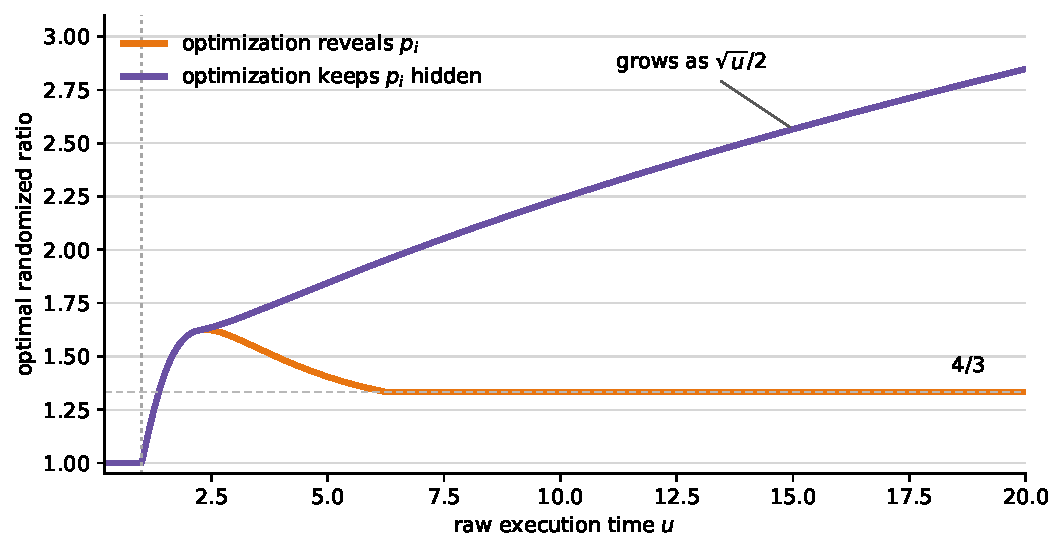
\includegraphics[width=0.78\textwidth]{blind_optimization_curve.pdf}
 \caption{Revealing $p_i$ keeps the randomized common-upper ratio bounded and
 eventually gives the $4/3$ plateau.  If optimization changes the processing
 time but does not reveal it before execution, the exact ratio instead grows
 as $\sqrt u/2$.}
 \label{fig:bo-comparison}
\end{figure}

The hard distribution explains the separation.  Most jobs have optimized
length zero, while a carefully chosen small fraction have length $u$.  Blind
optimization is attractive on average, so the online policy optimizes the
jobs.  It cannot recognize a long outcome before committing to it, and an
early long job delays many zeros.  The clairvoyant optimum optimizes the
zeros, runs the long jobs raw, and places them last.  In the revealing model,
by contrast, the same long outcomes can be deferred after their tests.  The
gap between the two curves therefore measures the scheduling value of the
revealed information itself.
